\PassOptionsToPackage{unicode=true}{hyperref} % options for packages loaded elsewhere
\PassOptionsToPackage{hyphens}{url}
%
\documentclass[ignorenonframetext,]{beamer}
\usepackage{pgfpages}
\setbeamertemplate{caption}[numbered]
\setbeamertemplate{caption label separator}{: }
\setbeamercolor{caption name}{fg=normal text.fg}
\beamertemplatenavigationsymbolsempty
% Prevent slide breaks in the middle of a paragraph:
\widowpenalties 1 10000
\raggedbottom
\setbeamertemplate{part page}{
\centering
\begin{beamercolorbox}[sep=16pt,center]{part title}
  \usebeamerfont{part title}\insertpart\par
\end{beamercolorbox}
}
\setbeamertemplate{section page}{
\centering
\begin{beamercolorbox}[sep=12pt,center]{part title}
  \usebeamerfont{section title}\insertsection\par
\end{beamercolorbox}
}
\setbeamertemplate{subsection page}{
\centering
\begin{beamercolorbox}[sep=8pt,center]{part title}
  \usebeamerfont{subsection title}\insertsubsection\par
\end{beamercolorbox}
}
\AtBeginPart{
  \frame{\partpage}
}
\AtBeginSection{
  \ifbibliography
  \else
    \frame{\sectionpage}
  \fi
}
\AtBeginSubsection{
  \frame{\subsectionpage}
}
\usepackage{lmodern}
\usepackage{amssymb,amsmath}
\usepackage{ifxetex,ifluatex}
\usepackage{fixltx2e} % provides \textsubscript
\ifnum 0\ifxetex 1\fi\ifluatex 1\fi=0 % if pdftex
  \usepackage[T1]{fontenc}
  \usepackage[utf8]{inputenc}
  \usepackage{textcomp} % provides euro and other symbols
\else % if luatex or xelatex
  \usepackage{unicode-math}
  \defaultfontfeatures{Ligatures=TeX,Scale=MatchLowercase}
\fi
% use upquote if available, for straight quotes in verbatim environments
\IfFileExists{upquote.sty}{\usepackage{upquote}}{}
% use microtype if available
\IfFileExists{microtype.sty}{%
\usepackage[]{microtype}
\UseMicrotypeSet[protrusion]{basicmath} % disable protrusion for tt fonts
}{}
\IfFileExists{parskip.sty}{%
\usepackage{parskip}
}{% else
\setlength{\parindent}{0pt}
\setlength{\parskip}{6pt plus 2pt minus 1pt}
}
\usepackage{hyperref}
\hypersetup{
            pdftitle={Government through Patronage},
            pdfauthor={Galileu Kim},
            pdfborder={0 0 0},
            breaklinks=true}
\urlstyle{same}  % don't use monospace font for urls
\newif\ifbibliography
\setlength{\emergencystretch}{3em}  % prevent overfull lines
\providecommand{\tightlist}{%
  \setlength{\itemsep}{0pt}\setlength{\parskip}{0pt}}
\setcounter{secnumdepth}{0}

% set default figure placement to htbp
\makeatletter
\def\fps@figure{htbp}
\makeatother

\usetheme{metropolis}
\setbeamertemplate{footline}[page number]{}

% packages
\usepackage{xcolor}
\usepackage{ragged2e}
\usepackage{setspace}
\usepackage{etoolbox}
\usepackage{caption}
\usepackage{graphicx}
\usepackage{float}
\usepackage{wrapfig}
\usepackage{blindtext}
\captionsetup[figure]{font=scriptsize} % set size of caption
\AtBeginEnvironment{knitrout}{\singlespacing}
\useoutertheme{infolines} % Alternatively: miniframes, infolines, split
\useinnertheme{circles}
\date[]{\today}

% colors
\definecolor{princeton}{rgb}{1.0, 0.6, 0.2} % princeton (primary)
\definecolor{arsenic}{rgb}{0.23, 0.27, 0.29}

\setbeamercolor{title}{fg=black}
\setbeamercolor{frametitle}{fg=white,bg=arsenic}
\setbeamercolor{section in head/foot}{fg=arsenic,bg=princeton}
\setbeamerfont{frametitle}{size=\Large}
\setbeamercolor{palette primary}{fg=white,bg=arsenic}
\setbeamercolor{palette secondary}{fg=arsenic,bg=princeton}
\setbeamercolor{palette tertiary}{fg=princeton,bg=arsenic}
\setbeamercolor{palette quaternary}{fg=princeton,bg=arsenic}
\setbeamercolor{structure}{fg=princeton} % itemize, enumerate, etc
\setbeamercolor{section in toc}{fg=arsenic} % TOC sections
\setbeamerfont{subtitle}{size=\small}

% override palette coloring with secondary
\setbeamercolor{subsection in head/foot}{bg=arsenic,fg=white}

% defining font
\usepackage[T1]{fontenc}

% Cabin
\usepackage[sfdefault,condensed]{cabin}

% Helvetica
%\usepackage[scaled]{helvet}
%\renewcommand\familydefault{\sfdefault}

% Inria Sans
%\usepackage[lining]{InriaSans}
%\renewcommand*\oldstylenums[1]{{\fontfamily{InriaSans-OsF}\selectfont #1}}
%% The font package uses mweights.sty which has som issues with the
%% \normalfont command. The following two lines fixes this issue.
%\let\oldnormalfont\normalfont
%\def\normalfont{\oldnormalfont\mdseries}

% FiraSans
%\usepackage[sfdefault]{FiraSans}
%\renewcommand*\oldstylenums[1]{{\firaoldstyle #1}}
%\usepackage{ragged2e}

% aesthetics
\setbeamersize{text margin left=10mm,text margin right=10mm}

% source command
\newcommand{\source}{\footnotesize\textcolor{black!25}}

% suppress section slides
\AtBeginPart{}
\AtBeginSubsection{}
\AtBeginSection{}
\setlength{\emergencystretch}{0em}
\setlength{\parskip}{0pt}

\title{Government through Patronage}
\providecommand{\subtitle}[1]{}
\subtitle{Bargaining for Education in Decentralized Brazil}
\author{Galileu Kim}
\providecommand{\institute}[1]{}
\institute{Princeton University}
\date{}

\begin{document}
\frame{\titlepage}

\begin{frame}{Education: a global perspective}
\protect\hypertarget{education-a-global-perspective}{}

\begin{itemize}
\tightlist
\item
  Children across the world rely on governments for education.
\item
  Access improved significantly over the past decades.
\item
  Improvements in quality remain a challenge.
\item
  ``Schooling does not always lead to learning. Worldwide, there are
  more non-learners in school than out of school.''

  \begin{itemize}
  \item
    \source{UNICEF.}
  \end{itemize}
\end{itemize}

\end{frame}

\begin{frame}{Global education}
\protect\hypertarget{global-education}{}

\begin{center}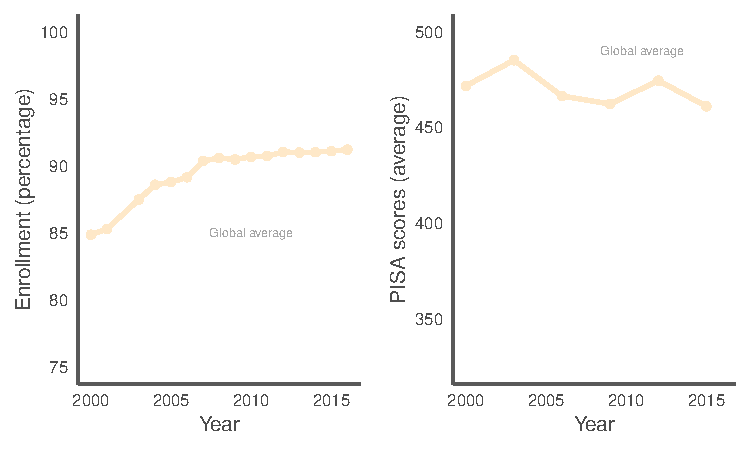
\includegraphics[width=240px]{plots/plot_global_1} \end{center}

\end{frame}

\begin{frame}{Education in Brazil}
\protect\hypertarget{education-in-brazil}{}

\begin{center}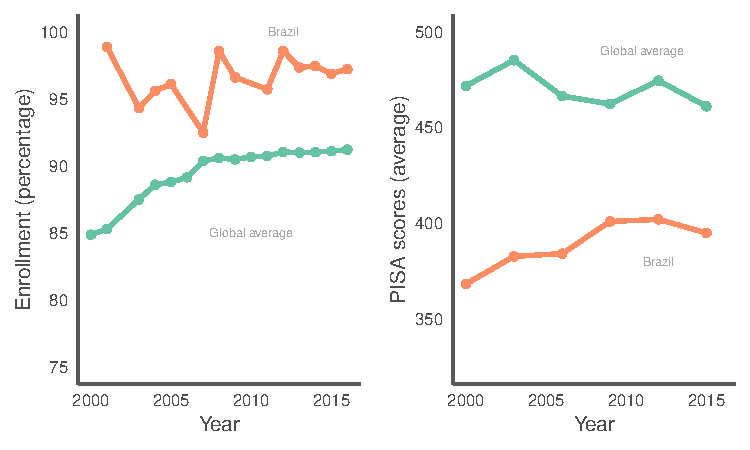
\includegraphics[width=240px]{plots/plot_global_2} \end{center}

\end{frame}

\begin{frame}{A domestic challenge}
\protect\hypertarget{a-domestic-challenge}{}

\begin{itemize}
\tightlist
\item
  Each country faces a particular set of challenges.

  \begin{itemize}
  \tightlist
  \item
    Widespread institutional reforms make cases comparable.
  \end{itemize}
\item
  Decentralization: subnational politicians have direct impact on public
  services.

  \begin{itemize}
  \item
    \source{Falleti 2010, Arretche 2017.}
  \end{itemize}
\item
  Quality of education varies along subnational lines.
\end{itemize}

\end{frame}

\begin{frame}{Mapping domestic inequality}
\protect\hypertarget{mapping-domestic-inequality}{}

\begin{figure}

{\centering 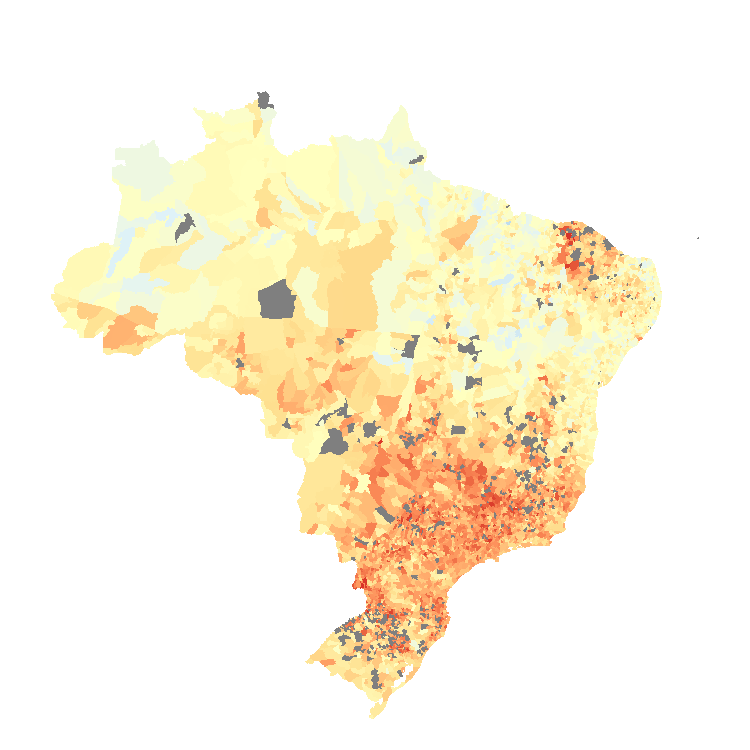
\includegraphics[width=180px]{plots/saeb_map} 

}

\caption{Municipal variation in the quality of education (2015). Polygons represent municipalities, warmer colors indicate higher municipal average in standardized test scores.}\label{fig:unnamed-chunk-3}
\end{figure}

\end{frame}

\begin{frame}{Findings}
\protect\hypertarget{findings}{}

\begin{itemize}
\tightlist
\item
  Decentralization delegates management over personnel.

  \begin{itemize}
  \tightlist
  \item
    Mayors and legislators have competing claims.
  \end{itemize}
\item
  Mayors allocate public sector jobs to gain legislative support.

  \begin{itemize}
  \tightlist
  \item
    Increased control by the executive reduces patronages.
  \end{itemize}
\item
  Bureaucratic turnover has negative effects on education.

  \begin{itemize}
  \tightlist
  \item
    Students perform worse on standardized exams.
  \end{itemize}
\end{itemize}

\end{frame}

\begin{frame}{Contribution}
\protect\hypertarget{contribution}{}

\begin{itemize}
\tightlist
\item
  Growing literature on the politics of personnel and public services.

  \begin{itemize}
  \item
    \source{Pepinsky 2013, Finan et al. 2015, Akhtari et al. 2017.}
  \end{itemize}
\item
  Interaction between political elites in local government.

  \begin{itemize}
  \item
    \source{Klasnja and Titiunik 2017, Novaes 2019.}
  \end{itemize}
\item
  Effect of competition in weakly institutionalized countries.

  \begin{itemize}
  \item
    \source{Gottlieb and Kosec 2019.}
  \end{itemize}
\end{itemize}

\end{frame}

\begin{frame}{Outline}
\protect\hypertarget{outline}{}

\singlespacing

\tableofcontents

\end{frame}

\hypertarget{related-literature}{%
\section{Related literature}\label{related-literature}}

\begin{frame}{Bureaucracy and public goods provision}
\protect\hypertarget{bureaucracy-and-public-goods-provision}{}

\begin{itemize}
\tightlist
\item
  Initial emphasis on industrialization and the developmental state.

  \begin{itemize}
  \item
    \source{Johnson 1982, Kohli 2004.}
  \end{itemize}
\item
  Political control can make bureaucracies deliver better public
  services.

  \begin{itemize}
  \item
    \source{Toral 2018, Shaffler 2016, Gulzar and Pasquale 2017.}
  \end{itemize}
\item
  Analyze who are the politicians managing bureaucracies.

  \begin{itemize}
  \tightlist
  \item
    And who do they govern with.
  \end{itemize}
\end{itemize}

\end{frame}

\begin{frame}{Presidential coalitionism and patronage}
\protect\hypertarget{presidential-coalitionism-and-patronage}{}

\begin{itemize}
\tightlist
\item
  Executive and legislators reshape policy and bureaucratic
  institutions.

  \begin{itemize}
  \item
    \source{Cameron and McCarty 2004, McCarty 2004.}
  \end{itemize}
\item
  Presidential coalitionism.

  \begin{itemize}
  \item
    Mayor (president) builds a coalition by allocating cabinet positions
    to city councilors (Congress members
  \item
    \source{Raile et al. 2011, Amorim Neto 2000.}
  \end{itemize}
\item
  Jobs allocated to city councilors.

  \begin{itemize}
  \tightlist
  \item
    ``City councilors knocked on my door with\ldots{}people they wanted
    me to hire.'' \source{- former mayor of S.}
  \end{itemize}
\end{itemize}

\end{frame}

\begin{frame}{Bureaucratic turnover and inexperienced education}
\protect\hypertarget{bureaucratic-turnover-and-inexperienced-education}{}

\begin{itemize}
\tightlist
\item
  Staff rotation induces negative productivity shock.

  \begin{itemize}
  \item
    \source{Gailmard and Patty 2007.}
  \end{itemize}
\item
  Students taught by inexperienced teachers and principals learn less.

  \begin{itemize}
  \item
    \source{Clotfelter et al. 2007, Akhtari et al. 2017.}
  \end{itemize}
\item
  ``I am aware that the position is temporary. Especially because it is
  a political position, decided by the administration.''
  \source{- school principal in municipality I.}
\end{itemize}

\end{frame}

\hypertarget{theory}{%
\section{Theory}\label{theory}}

\begin{frame}{Theory}
\protect\hypertarget{theory-1}{}

\begin{itemize}
\tightlist
\item
  Model the executive decision over patronage allocation during
  government.

  \begin{itemize}
  \tightlist
  \item
    Mayors need to coopt a winning coalition in the legislature.
  \end{itemize}
\item
  Trade-off between patronage and quality of public services.

  \begin{itemize}
  \tightlist
  \item
    Probability of reelection vs.~governance.
  \end{itemize}
\item
  From pre-electoral bargains with brokers to administrative term.

  \begin{itemize}
  \item
    \source{Stokes et al. 2013, Robinson and Verdier 2013.}
  \end{itemize}
\end{itemize}

\end{frame}

\begin{frame}{Prediction}
\protect\hypertarget{prediction}{}

\begin{itemize}
\tightlist
\item
  Mayors with a larger coalition engage in less patronage.

  \begin{itemize}
  \tightlist
  \item
    Executive prioritizes cheap votes.
  \end{itemize}
\item
  Legislators who already formed an electoral alliance with the
  government.

  \begin{itemize}
  \item
    \source{Groseclose and Snyder 1996, Banks 2000.}
  \end{itemize}
\item
  Controlling less seats makes buying a majority more expensive.

  \begin{itemize}
  \tightlist
  \item
    Indifferent or opposition legislators demand more jobs.
  \end{itemize}
\end{itemize}

\end{frame}

\hypertarget{institutional-context}{%
\section{Institutional context}\label{institutional-context}}

\begin{frame}{Public education in Brazil}
\protect\hypertarget{public-education-in-brazil}{}

\begin{itemize}
\tightlist
\item
  Over 20 million students enrolled in municipal schools.

  \begin{itemize}
  \tightlist
  \item
    1.2 million public teachers and 100 thousand school principals.
  \end{itemize}
\item
  Primary education managed by municipal governments.

  \begin{itemize}
  \tightlist
  \item
    Personnel decisions centralized by the executive, subject to
    legislative influence.
  \end{itemize}
\item
  ``We are invited to work at the school by the department of education,
  with the city councilor\ldots{}appointing people they think have the
  necessary qualifications.'' \source{- school principal A.}
\end{itemize}

\end{frame}

\begin{frame}{Enrollment by administrative level}
\protect\hypertarget{enrollment-by-administrative-level}{}

\begin{figure}

{\centering 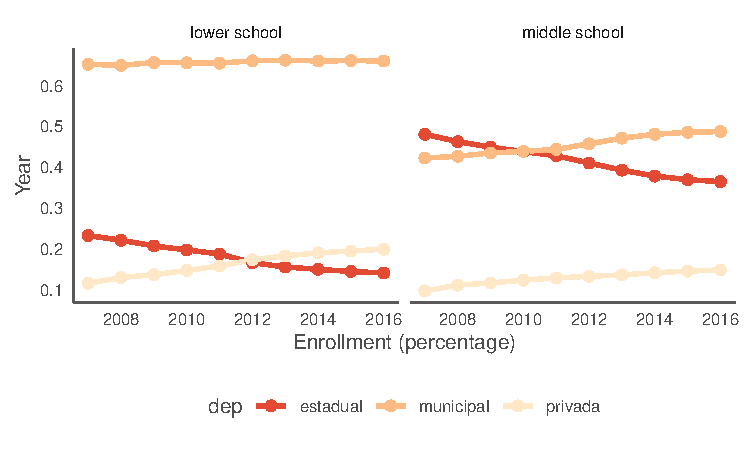
\includegraphics[width=230px]{plots/enrollment_dep} 

}

\caption{A decentralized system. Lower school education is primarily under the responsibility of municipalities.}\label{fig:unnamed-chunk-4}
\end{figure}

\end{frame}

\begin{frame}{Local government}
\protect\hypertarget{local-government}{}

\begin{itemize}
\tightlist
\item
  Local politicians elected for four year terms, with reelection.

  \begin{itemize}
  \tightlist
  \item
    5 thousand mayors and over 50 thousand city councilors.
  \end{itemize}
\item
  Executive responsible for delivering public services.

  \begin{itemize}
  \tightlist
  \item
    City council gives budgetary approval and legal oversight.
  \end{itemize}
\item
  Executive coalitions declared during electoral campaign.

  \begin{itemize}
  \tightlist
  \item
    Political alliance for electoral campaign and during mayoral term.
  \end{itemize}
\end{itemize}

\end{frame}

\hypertarget{research-design-and-data}{%
\section{Research design and data}\label{research-design-and-data}}

\begin{frame}{Research design}
\protect\hypertarget{research-design}{}

\begin{itemize}
\item
  Bureaucratic turnover \(\rightarrow\) student learning. \begin{align*}
  \text{test score}_{isjt} &= \beta_1 \text{turnover}_{isjt} + \beta_2 \text{grade}_{isjt} +\beta_3 \text{turnover}_{isjt} \times \text{grade}_{isjt} + \\ 
  &\psi X_{isjt} + \phi V_{sjt} +\zeta W_{jt}+ \alpha_k + \delta_t + \epsilon_{isjt}
  \end{align*}
\item
  Model specification: hierarchical linear modeling with heterogeneous
  effect by grade and state-year fixed effects.

  \begin{itemize}
  \tightlist
  \item
    Outcome of interest: average student test scores at the classroom
    level.
  \item
    Treatment: (1) teacher and school principal turnover, (2) teacher
    turnover index.
  \item
    Unit of analysis: classroom.
  \end{itemize}
\end{itemize}

\end{frame}

\begin{frame}{Research design}
\protect\hypertarget{research-design-1}{}

\begin{itemize}
\item
  Executive coalition \(\rightarrow\) bureaucratic turnover.
  \[\text{turnover}_{sjt} = \gamma \text{coalition seats}_{jt} + \mu P_{jt} + \zeta W_{jt}+ \alpha_k + \delta_t + \epsilon_{jt}\]
\item
  Model specification: (1) logistic regression, (2) linear model with
  state-year fixed effects.

  \begin{itemize}
  \tightlist
  \item
    Outcome of interest: (1) hiring/dismissal of teacher/school
    principal, (2) proportion of dismissal and hiring.
  \item
    Treatment: share of legislative seats held by executive coalition.
  \item
    Unit of analysis: (1) individual bureaucrat, (2) municipal
    bureaucracy.
  \end{itemize}
\end{itemize}

\end{frame}

\begin{frame}{Data}
\protect\hypertarget{data}{}

\begin{itemize}
\tightlist
\item
  Student learning.

  \begin{itemize}
  \tightlist
  \item
    SAEB (2007 - 2015): national test scores for 5 million students (5th
    and 9th grades).
  \item
    SPAECE (2007 - 2018): state test scores for 400 thousand students
    (2nd, 5th and 9th grades).
  \end{itemize}
\item
  Educational staff.

  \begin{itemize}
  \tightlist
  \item
    National school census (1995 - 2016): annual census of 100 thousand
    schools.
  \item
    RAIS (1985 - 2015): annual employment data on school principals and
    teachers (over 1 million per year).
  \end{itemize}
\item
  Fieldwork.

  \begin{itemize}
  \tightlist
  \item
    Interviews conducted in summmers of 2018 and 2019 in Brazil.
  \item
    Mayors, secretaries of education, school principals and teachers.
  \end{itemize}
\end{itemize}

\end{frame}

\begin{frame}{Bureaucratic turnover by department}
\protect\hypertarget{bureaucratic-turnover-by-department}{}

\begin{figure}

{\centering 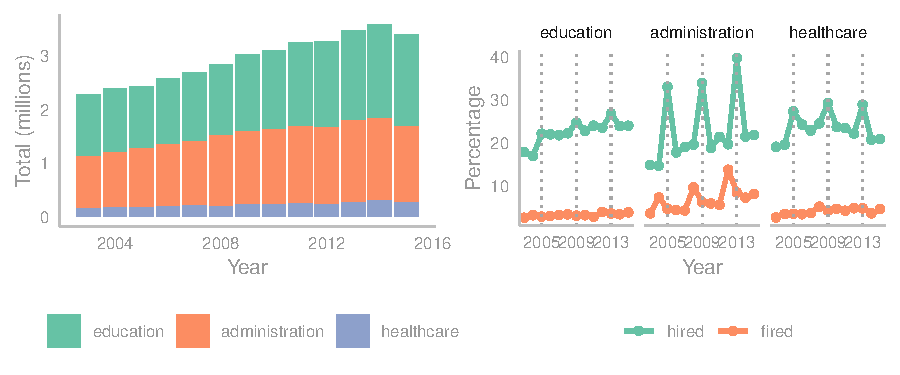
\includegraphics[width=230px]{plots/turnover_category} 

}

\caption{Municipal bureaucracies. Total number of bureaucrats and hiring/dismissal rates for bureaucratic staff over time. Disaggregated by department.}\label{fig:staff}
\end{figure}

\end{frame}

\begin{frame}{Results}
\protect\hypertarget{results}{}

\begin{itemize}
\tightlist
\item
  Staff turnover has negative effects on student learning.

  \begin{itemize}
  \tightlist
  \item
    Robust to different turnover and standardized exam specifications.
  \end{itemize}
\item
  Increase in patronage in municipalities with lower share of
  executive-held seats.

  \begin{itemize}
  \tightlist
  \item
    Similar pattern for different turnover specifications (hiring,
    dismissal and turnover).
  \end{itemize}
\end{itemize}

\end{frame}

\begin{frame}{Staff turnover and student test scores: SAEB and SPAECE}
\protect\hypertarget{staff-turnover-and-student-test-scores-saeb-and-spaece}{}

\begin{table}[t]
  \centering
  \resizebox*{!}{\height}{%
  
% Table created by stargazer v.5.2.2 by Marek Hlavac, Harvard University. E-mail: hlavac at fas.harvard.edu
% Date and time: Fri, Jun 12, 2020 - 01:12:19 PM
\begingroup 
\small 
\begin{tabular}{@{\extracolsep{5pt}}lcccccccc} 
\\[-1.8ex]\hline 
\hline \\[-1.8ex] 
 & \multicolumn{8}{c}{Student learning} \\ 
\cline{2-9} 
 & \multicolumn{4}{c}{SAEB test score} & \multicolumn{2}{c}{SPAECE test score} &  &  \\ 
\\[-1.8ex] & (1) & (2) & (3) & (4) & (5) & (6) & (7) & (8)\\ 
\hline \\[-1.8ex] 
 Turnover index & $-$0.073$^{***}$ & $-$0.049$^{***}$ &  &  &  &  & $-$0.054$^{***}$ & $-$0.057$^{***}$ \\ 
  & (0.008) & (0.017) &  &  &  &  & (0.015) & (0.015) \\ 
  Turnover index $\times$ Grade 9 &  &  & $-$0.050$^{***}$ & $-$0.031$^{**}$ &  &  &  &  \\ 
  &  &  & (0.005) & (0.013) &  &  &  &  \\ 
  Teacher experience (2 years) &  &  & 0.028 & $-$0.087$^{**}$ &  &  &  &  \\ 
  &  &  & (0.018) & (0.043) &  &  &  &  \\ 
  Teacher experience (10 years) &  &  &  &  & $-$0.160$^{***}$ & $-$0.120$^{***}$ &  &  \\ 
  &  &  &  &  & (0.006) & (0.014) &  &  \\ 
  School principal experience (2 years) &  &  &  &  & 0.021$^{**}$ & 0.004 &  &  \\ 
  &  &  &  &  & (0.010) & (0.024) &  &  \\ 
  School principal experience (10 years) & 0.004$^{***}$ & 0.003 &  &  &  &  &  &  \\ 
  & (0.001) & (0.003) &  &  &  &  &  &  \\ 
  saeb\_principal\_experienceless than 2 years:grade\_level &  &  & $-$0.003$^{***}$ & $-$0.009$^{***}$ &  &  &  &  \\ 
  &  &  & (0.001) & (0.002) &  &  &  &  \\ 
  saeb\_principal\_experiencemore than 10:grade\_level &  &  & 0.020$^{***}$ & 0.033$^{***}$ &  &  &  &  \\ 
  &  &  & (0.003) & (0.007) &  &  &  &  \\ 
  saeb\_teacher\_work\_schoolless than 2:grade\_level &  &  &  &  & 0.007$^{***}$ & 0.005$^{**}$ &  &  \\ 
  &  &  &  &  & (0.001) & (0.002) &  &  \\ 
  saeb\_teacher\_work\_schoolmore than 10:grade\_level &  &  &  &  & $-$0.002 & $-$0.003 &  &  \\ 
  &  &  &  &  & (0.002) & (0.004) &  &  \\ 
  turnover\_index:grade9 &  &  &  &  &  &  & 0.062$^{***}$ & 0.065$^{***}$ \\ 
  &  &  &  &  &  &  & (0.018) & (0.018) \\ 
 \hline \\[-1.8ex] 
Controls & \_ & \checkmark & \_ & \checkmark & \_ & \checkmark &  &  \\ 
Observations & 165,013 & 26,075 & 1,135,748 & 164,808 & 837,248 & 163,984 & 2,860 & 2,860 \\ 
\hline 
\hline \\[-1.8ex] 
\textit{Note:}  & \multicolumn{8}{r}{$^{*}$p$<$0.1; $^{**}$p$<$0.05; $^{***}$p$<$0.01} \\ 
\end{tabular} 
\endgroup 
%
  }
  \caption{\textbf{Bureaucratic turnover and student learning.} Higher turnover in teachers and principals reduce student learning. All models include year and state fixed effects.}
  \label{tbl:hlm_mods}
\end{table}

\end{frame}

\begin{frame}{Staff turnover and student test scores: SAEB and SPAECE}
\protect\hypertarget{staff-turnover-and-student-test-scores-saeb-and-spaece-1}{}

\begin{figure}

{\centering 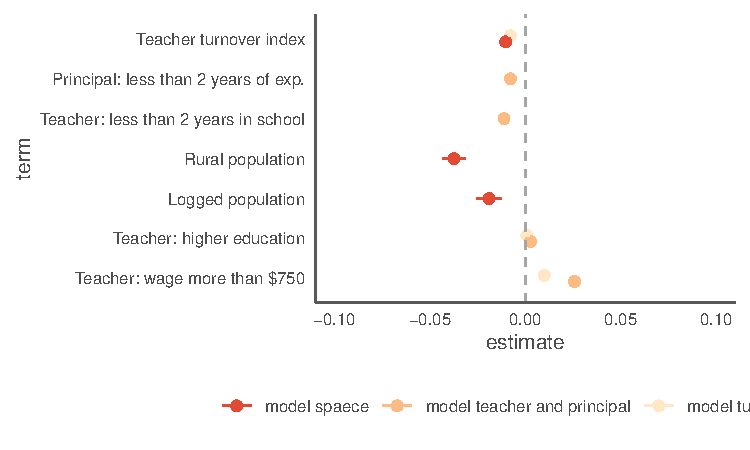
\includegraphics[width=210px]{plots/turnover_fit} 

}

\caption{Relative impact of bureaucratic turnover. Point estimates and confidence intervals retrieved from models with controls.}\label{fig:unnamed-chunk-5}
\end{figure}

\end{frame}

\begin{frame}{Executive coalition and staff turnover}
\protect\hypertarget{executive-coalition-and-staff-turnover}{}

\begin{table}[t]
  \centering
  \resizebox*{!}{\height}{%
  
% Table created by stargazer v.5.2.2 by Marek Hlavac, Harvard University. E-mail: hlavac at fas.harvard.edu
% Date and time: Fri, Jul 03, 2020 - 12:37:34 PM
\begingroup 
\small 
\begin{tabular}{@{\extracolsep{5pt}}lcccccc} 
\\[-1.8ex]\hline 
\hline \\[-1.8ex] 
 & \multicolumn{6}{c}{Outcome} \\ 
\cline{2-7} 
 & \multicolumn{2}{c}{Turnover index (municipal)} & \multicolumn{2}{c}{Hires (municipal)} & \multicolumn{2}{c}{Hires (individual)} \\ 
\\[-1.8ex] & (1) & (2) & (3) & (4) & (5) & (6)\\ 
\hline \\[-1.8ex] 
 Share of legislative seats & $-$0.026$^{***}$ & $-$0.053$^{***}$ & $-$0.028$^{***}$ & $-$0.030$^{***}$ & $-$0.040$^{***}$ & $-$0.047$^{***}$ \\ 
  & (0.008) & (0.007) & (0.006) & (0.006) & (0.002) & (0.003) \\ 
  School principal &  &  & $-$0.252$^{***}$ & $-$0.245$^{***}$ & $-$0.222$^{***}$ & $-$0.386$^{***}$ \\ 
  &  &  & (0.015) & (0.017) & (0.013) & (0.015) \\ 
  Executive share of seats X School principal &  &  & $-$0.014 & $-$0.022$^{**}$ & $-$0.016 & $-$0.128$^{***}$ \\ 
  &  &  & (0.011) & (0.010) & (0.013) & (0.014) \\ 
 \hline \\[-1.8ex] 
Controls &  & \checkmark &  & \checkmark &  & \checkmark \\ 
State and year FE & \checkmarck & \checkmarck & \checkmarck & \checkmarck & \checkmarck & \checkmarck \\ 
Observations & 2,591,629 & 1,632,748 & 61,983 & 61,983 & 1,303,399 & 1,303,399 \\ 
R$^{2}$ & 0.027 & 0.045 & 0.184 & 0.296 &  &  \\ 
\hline 
\hline \\[-1.8ex] 
\textit{Note:}  & \multicolumn{6}{r}{$^{*}$p$<$0.1; $^{**}$p$<$0.05; $^{***}$p$<$0.01} \\ 
\end{tabular} 
\endgroup 
%
  }
  \caption{{\bf Executive coalitions and staff turnover.} An increase in the share of legislative seats held by the mayoral coalition decrease the amount of turnover for teachers and school principals, including hires or dismissals. Models 1, 3, and 5 include year and state fixed effects.}
  \label{tbl:turnover}
\end{table}

\end{frame}

\begin{frame}{Executive coalition and staff turnover}
\protect\hypertarget{executive-coalition-and-staff-turnover-1}{}

\begin{figure}

{\centering 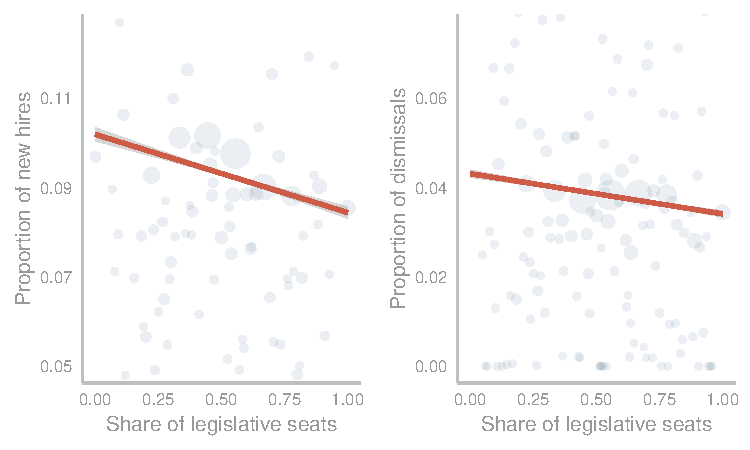
\includegraphics[width=230px]{plots/plot_pred} 

}

\caption{Predicted and actual values for bureaucratic turnover. The line graph plots the predicted proportion of educational staff hired or firede. Circles' size is proportional to the number of observations contained in the data.}\label{fig:unnamed-chunk-6}
\end{figure}

\end{frame}

\hypertarget{conclusion}{%
\section{Conclusion}\label{conclusion}}

\begin{frame}{Conclusion}
\protect\hypertarget{conclusion-1}{}

\begin{itemize}
\tightlist
\item
  Subnational political actors manage public services.

  \begin{itemize}
  \tightlist
  \item
    Political elites interact and negotiate with one another.
  \end{itemize}
\item
  Bureaucratic turnover results from executives coopting legislators.

  \begin{itemize}
  \tightlist
  \item
    Negative downstream consequences for the quality of education.
  \end{itemize}
\item
  Is political competition welfare enhancing for citizen?

  \begin{itemize}
  \tightlist
  \item
    Future research can theorize on how heterogeneous political elites
    reshape governments.
  \end{itemize}
\end{itemize}

\end{frame}

\begin{frame}{Thank you!}
\protect\hypertarget{thank-you}{}

If you have any comments/suggestions:

\fontfamily{cmtt}\selectfont \href{mailto:galileuk@princeton.edu}{\nolinkurl{galileuk@princeton.edu}}

\appendix

\end{frame}

\end{document}
